% !TEX program = xelatex
%%%%%%%%%%%%%%%%%%%%%%%%

\documentclass[11pt,aspectratio=169]{beamer} % 11pt is default
\usetheme{metropolis} % [progressbar=frametitle]
\setbeamercolor{background canvas}{bg=white}
\setbeamertemplate{caption}{\insertcaption} 
\setbeamersize{text margin left=2em,text margin right=2em}
\setbeamertemplate{frame footer}{\vspace{-5pt}}

\usepackage[round]{natbib}
\usepackage{amsmath}
\usepackage{mathtools}
\usepackage[group-minimum-digits=4,group-separator={,}]{siunitx}
\usepackage{graphicx}
\usepackage{wrapfig}
\usepackage{multimedia}

\usepackage{tikz}
\usetikzlibrary{backgrounds}
\usetikzlibrary{arrows,shapes}
\usetikzlibrary{tikzmark}
\usetikzlibrary{calc}
\usepackage[dvipsnames]{xcolor}

\usepackage[skins,theorems]{tcolorbox}
\usepackage{pdfpages}
\usepackage{colortbl}
\usepackage{changepage}
\usepackage{booktabs}
\usepackage{makecell}
\usepackage{setspace}
\usepackage{algorithm}
\usepackage[noend]{algpseudocode}
\usepackage{subcaption}
\usepackage[framemethod=TikZ]{mdframed}
\usepackage{xspace}

\usepackage{annotate-equations}

% Shortcut for beamer frames
\newcommand{\bframe}[2][c]{\begin{frame}[#1]{#2}}
\newcommand{\eframe}{\end{frame}} % \eframe causes problems for some reason

% Shortcut for bold text
\newcommand{\fat}[1]{\textbf{#1}}

% Boxing items on slide
\newcommand{\Cboxed}[2]{\colorlet{currentcolor}{.}{\color{#1}\fbox{\color{currentcolor}#2}}} %create coloured box around equation

% checkmark and xmark
\usepackage{pifont}
\newcommand{\cmark}{\ding{51}}%
\newcommand{\xmark}{\ding{55}}%

% Highlighting text in orange
\newcommand{\e}[1]{\alert{#1}}

% Underline
\newcommand{\uline}[1]{\underline{#1}}

% Include figure
\newcommand{\imgw}[2]{\includegraphics[width=#2\textwidth]{#1}} % \imgw{file}{height-scale}
\newcommand{\imgh}[2]{\includegraphics[height=#2\textheight]{#1}} % \imgh{file}{width-scale}

% Shortcut for latex commands
\newcommand{\blist}{\vspace{-3pt}\begin{list}{\raisebox{1pt}{\small$\bullet$}}{\leftmargin=13pt\itemsep=4pt}}
\newcommand{\blisttab}{\vspace{5pt}\blist}
\newcommand{\elisttab}{\end{list}}
\newcommand{\listtab}{\\[3pt] $\Rightarrow$ }
\newcommand{\elist}{\end{list}\vspace{5pt}}
\newcommand{\bblock}[1]{\metroset{block=fill}\begin{block}{#1}}
\newcommand{\eblock}{\end{block}}
\newcommand{\bmath}[1][0]{\begin{equation*}\hspace{#1em}}
\newcommand{\emath}{\end{equation*}}
\newcommand{\bcol}{\begin{columns}}
\newcommand{\col}[1]{\column{#1\textwidth}}
\newcommand{\tcol}[1]{\column[T]{#1\textwidth}}
\newcommand{\ecol}{\end{columns}}
\newcommand{\place}[4]{\begin{textblock}{#3}(#1,#2) #4 \end{textblock}} % \place{x}{y}{width}{text}
\newcommand{\placeframed}[4]{\place{#1}{#2}{#3}{\fbox{\parbox{#3em}{#4}}}}
\newcommand{\placeimg}[4]{\place{#1}{#2}{#3}{\imgw{#4}{1}}} % \placeimg{x}{y}{width}{file}
\newcommand{\videolink}[2]{\movie[externalviewer]{{\bf Video:} #1}{videos/#2}} % \videolink{title}{file}
\newcommand{\btab}[1]{\begin{tabular}{#1}}
\newcommand{\etab}{\end{tabular}}
\newcommand{\balgo}[2][1.3]{{#2:} \\[5pt] \begin{algorithmic}[1] \linespread{#1}\selectfont}
\newcommand{\ealgo}{\end{algorithmic}}
\renewcommand{\algorithmicloop}{\textbf{repeat:}}
\newcommand{\cred}{\cellcolor{red!25}}
\newcommand{\cgreen}{\cellcolor{green!25}}

% Shortcut for commonly used math symbols
\newcommand{\condpr}[2]{\text{Pr}\hspace{-1pt}\left\{ #1 \ \mid \ #2 \right\}}
\newcommand{\exarg}[2]{\mathbb{E}_{#1}\hspace{-2pt}\left[ #2 \right]}
\newcommand{\exnoarg}[1]{\mathbb{E}_{#1}}
\NewDocumentCommand\ex{ m g }{
	\IfNoValueTF{#2}{\exnoarg{#1}}{\exarg{#1}{#2}}
}
\newcommand{\der}[2]{\frac{\partial #1}{\partial #2}}
\newcommand{\stats}{\mathcal{S}}
\newcommand{\acts}{\mathcal{A}}
\newcommand{\rews}{\mathcal{R}}
\newcommand{\eps}{\mathcal{E}}
\newcommand{\ver}{\,\vert\,}
\newcommand{\vhat}{\hat{v}}
\newcommand{\qhat}{\hat{q}}
% \newcommand{\para}{\textbf{w}}
\newcommand{\feats}{\textbf{x}}
\newcommand{\elig}{\textbf{z}}
\newcommand{\gradient}{\nabla}
\newcommand{\outline}{Lecture Outline}
\newcommand{\reading}{Reading}
\newcommand{\h}[1]{\emph{#1}}

\emph
% \newcommand{\lindex}[1]{%
% 	\lowercase{\def\temp{#1}%
% 	\expandafter\index\expandafter{\temp}%
% }

\newcommand{\indx}[1]{\index{#1}}
\newcommand{\hind}[1]{\h{#1}\lindex{#1}}

% Set of real numbers
\newcommand{\R}{\mathbb{R}}
% Proportional to
% Transpose of a vector x
\newcommand{\vectranspose}[1]{#1^\top}
% Transpose of a matrix X
\newcommand{\mattranspose}[1]{#1^\top}
% Probability
\newcommand{\pr}{\text{Pr}}
% Conditional probability of x given y
\newcommand{\cpr}[2]{\pr( #1 \mid #2 )}
% x sampled according to probability distribution p
\newcommand{\sampled}[2]{#1 \sim #2}
% Assign value y to variable x
\newcommand{\assign}[2]{#1 \gets #2}
% Training data set
\newcommand{\data}{\mathcal{D}}
% Concatenation of inputs a, b, c, ...
\newcommand{\con}[1]{\langle #1 \rangle}
% array with bracket
\newcommand{\bra}[2]{\left[ \begin{array}{#1} #2 \end{array} \right]}
% Indicator function: returns 1 if x is true, otherwise returns 0
\newcommand{\ind}[1]{[#1]_1}

% common way of referring to places
\newcommand{\seehere}[1]{(\cref{#1})}

% shortcut text commands
\newcommand{\rl}{RL\xspace}
\newcommand{\marl}{MARL\xspace}
\newcommand{\ctde}{CTDE\xspace}
\newcommand{\sa}{single-agent\xspace}
\newcommand{\ma}{multi-agent\xspace}
\newcommand{\Ma}{Multi-agent\xspace}
\newcommand{\mas}{multi-agent system\xspace}
\newcommand{\stat}{stationarity\xspace}
\newcommand{\nonstat}{non-stationarity\xspace}
\newcommand{\pg}{policy gradient\xspace}
\newcommand{\vb}{value-based\xspace}
\newcommand{\pbt}{population-based training\xspace}
\newcommand{\psro}{policy space response oracles\xspace}
\newcommand{\Psro}{Policy space response oracles\xspace}
\newcommand{\sct}{\emph{StarCraft~II}\xspace}
\newcommand{\as}{AlphaStar\xspace}
\newcommand{\az}{AlphaZero\xspace}
\newcommand{\lbf}{level-based foraging\xspace}
\newcommand{\Lbf}{Level-based foraging\xspace}
\newcommand{\nfg}{normal-form game\xspace}
\newcommand{\nfgs}{normal-form games\xspace}
\newcommand{\Nfg}{Normal-form game\xspace}
\newcommand{\Nfgs}{Normal-form games\xspace}
\newcommand{\rps}{Rock-Paper-Scissors\xspace}
\newcommand{\pd}{Prisoner's Dilemma\xspace}
\newcommand{\survey}[4]{\noindent #1 (#4). ``#2.'' In: {\it #3}. \\}
\newcommand{\nashprob}{\textsc{Nash}\xspace}
\newcommand{\eol}{\textsc{End-of-Line}\xspace}
\newcommand{\ul}[1]{\underline{#1}}
\newcommand\norm[1]{\lVert#1\rVert}
\newcommand{\qlearn}{Q-learning\xspace}
\newcommand{\sarsa}{Sarsa\xspace}
\newcommand{\bayes}{Bayesian\xspace}
\newcommand{\bellman}{Bellman\xspace}
\newcommand{\markov}{Markov\xspace}
\newcommand{\pareto}{Pareto\xspace}
\newcommand{\boltzmann}{Boltzmann\xspace}
\newcommand{\mc}{Monte Carlo\xspace}
\newcommand{\nash}{Nash\xspace}
\newcommand{\ppad}{PPAD}
\newcommand{\dqn}{deep Q-networks\xspace}
\newcommand{\reinforce}{REINFORCE\xspace}
\newcommand{\qmix}{QMIX\xspace}
\newcommand{\qtran}{QTRAN\xspace}
\newcommand{\adam}{Adam\xspace}
\newcommand{\nret}{{$N$}-step returns\xspace}

% COMMANDS FOR COMMON NOTATION

% agent set
% state space
\newcommand{\St}{S}
\newcommand{\Stterm}{\bar{\St}}
% state
\newcommand{\st}{s}
\newcommand{\sth}{\hat{\st}}
% observation space
\newcommand{\Ob}{O}

% observation
\newcommand{\ob}{o}

% joint observation
\newcommand{\job}{o}
% action space
\newcommand{\Ac}{A}

% action
\newcommand{\ac}{a}
\newcommand{\ach}{\hat{\ac}}

% joint action
\newcommand{\jac}{a}
% reward
\newcommand{\rew}{r}
\newcommand{\rewh}{\hat{\rew}}
% centralised information
\newcommand{\ci}{z}

% initial state distribution

\newcommand{\instdist}{\mu}
% % state transition function

\newcommand{\Stf}{\mathcal{T}}
% % simulation/sampling model
\newcommand{\Stfsim}{\widehat{\Stf}}

% observation function
\newcommand{\Obf}{\mathcal{O}}

% reward function
\newcommand{\Rew}{\mathcal{R}}

% POLICIES, RETURNS, VALUES

% policy space
\newcommand{\Pol}{\Pi}

% policy
\newcommand{\pol}{\pi}
\newcommand{\poltil}{\tilde{\pol}}

% set of histories
\newcommand{\His}{H}
\newcommand{\Fhis}{\hat{\His}}
% history
\newcommand{\his}{h}

% full history
\newcommand{\fhis}{\hat{\his}}

% observation history extracted from full history
\newcommand{\obsext}{\sigma}

% discount factor
\newcommand{\dsc}{\gamma}

% return
\newcommand{\ret}{u}

% expected return for joint policy
\newcommand{\exret}{U}

% Agents
\newcommand{\Ag}{I}

% RL / MARL

% learning algorithm

\newcommand{\alg}{\mathbb{L}}

% empirical distribution/ average policy
\newcommand{\empdis}{\bar{\pol}}
\newcommand{\avgpol}{\bar{\pol}}
\newcommand{\agmod}{\hat{\pol}}
\newcommand{\Agmod}{\hat{\Pol}}
\newcommand{\agmodj}{agent model for agent $j$}

% best response
\newcommand{\br}{\textnormal{BR}}

% game value
\newcommand{\gval}{Value}

% value under agent model
\newcommand{\amval}{AV}

% regret
\newcommand{\regret}{Regret}
\newcommand{\avgreg}{\bar{R}}
% TD target
\newcommand{\target}{\mathcal{X}}
% step size (for gradient-based MARL in Chapter 5)
\newcommand{\step}{\kappa}


% DEEP LEARNING

% parameters
\newcommand{\para}{\theta}

% loss
\newcommand{\loss}{\mathcal{L}}
% batch
\newcommand{\batch}{\mathcal{B}}
\newcommand{\batchsize}{B}

% etnropy
\newcommand{\entropy}{\mathcal{H}}

% Create algorithm environment
\newcommand{\balg}[2]{
  \begin{algorithm}[H]
    \caption{#1}
    \label{alg:#2}
    \setstretch{1.1}
    \begin{algorithmic}[1]}

\newcommand{\ealg}{
    \end{algorithmic}
  \end{algorithm}}

% Argmin/ Argmax operators

\DeclareMathOperator*{\argmin}{arg\,min} 
\DeclareMathOperator*{\argmax}{arg\,max}

\makeatletter
\newenvironment{myitemize}{%
   \setlength{\topsep}{0pt}
   \setlength{\partopsep}{0pt}
   \renewcommand*{\@listi}{\leftmargin\leftmargini \parsep\z@ \topsep\z@ \itemsep\z@}
   \let\@listI\@listi
   \itemize
}{\enditemize}
\makeatother  

% define widebar for target parameters
\makeatletter
\newcommand*\rel@kern[1]{\kern#1\dimexpr\macc@kerna}
\newcommand*\widebar[1]{%
	\begingroup
	\def\mathaccent##1##2{%
		\rel@kern{0.8}%
		\overline{\rel@kern{-0.8}\macc@nucleus\rel@kern{0.2}}%
		\rel@kern{-0.2}%
	}%
	\macc@depth\@ne
	\let\math@bgroup\@empty \let\math@egroup\macc@set@skewchar
	\mathsurround\z@ \frozen@everymath{\mathgroup\macc@group\relax}%
	\macc@set@skewchar\relax
	\let\mathaccentV\macc@nested@a
	\macc@nested@a\relax111{#1}%
	\endgroup
}
\makeatother


% MATRIX GAMES

\newcolumntype{?}{!{\vrule width 1pt}}
\newcommand{\bhline}{\Xhline{1pt}}
\newcommand{\gametwo}[3]{
	\begin{tabular}{c?c|c}
		 & #1 \\
		\bhline
		#2    \\
		\hline
		#3    \\
	\end{tabular}
}
\newcommand{\gamethree}[4]{
	\begin{tabular}{c?c|c|c}
		 & #1 \\
		\bhline
		#2    \\
		\hline
		#3    \\
		\hline
		#4    \\
	\end{tabular}
}

\newcommand{\gamepd}{
    % \gametwo{C & D}{C & -1,-1 & -5,0}{D & 0,-5 & -3,-3}
	\begin{tabular}{c|c|c}
	& C & D \\
	\hline
	C & -1,-1 & -5,0 \\
	\hline
	D & 0,-5 & -3,-3
	\end{tabular}
}

\newcommand{\gamerps}{
    % \gamethree{R & P & S}{R & 0,0 & -1,1 & 1,-1}{P & 1,-1 & 0,0 & -1,1}{S & -1,1 & 1,-1 & 0,0}
	\begin{tabular}{c|c|c|c}
	& R & P & S \\
	\hline
	R & 0,0 & -1,1 & 1,-1 \\
	\hline
	P & 1,-1 & 0,0 & -1,1 \\
	\hline
	S & -1,1 & 1,-1 & 0,0
	\end{tabular}
}

\newcommand{\gamecoord}{
    % \gametwo{A & B}{A & 10 & 0}{B & 0 & 10}
	\begin{tabular}{c|c|c}
		& A & B \\
		\hline
		A & 10 & 0 \\
		\hline
		B & 0 & 10 \\
	\end{tabular}
}

\newcommand{\gamechicken}{
    % \gametwo{S & L}{S & 0,0 & 7,2}{L & 2,7 & 6,6}
	\begin{tabular}{c|c|c}
		& S & L \\
		\hline
		S & 0,0 & 7,2 \\
		\hline
		L & 2,7 & 6,6
	\end{tabular}
}

\newcommand{\gamestaghunt}{
    % \gametwo{S & H}{S & 4,4 & 0,3}{H & 3,0 & 2,2}
	\begin{tabular}{c|c|c}
		& S & H \\
		\hline
		S & 4,4 & 0,3 \\
		\hline
		H & 3,0 & 2,2
	\end{tabular}
}

\newcommand{\gamebattle}{
    \begin{tabular}{c|c|c}
    & A & B \\
    \hline
    A & 10,7 & 2,2 \\
    \hline
    B & 0,0 & 7,10
    \end{tabular}
}

\newcommand{\gameepsne}{
    % \gametwo{C & D}{A & 100,100 & 0,0}{B & 1,2 & 1,1}
	\begin{tabular}{c|c|c}
		& C & D \\
		\hline
		A & 100,100 & 0,0 \\
		\hline
		B & 1,2 & 1,1
	\end{tabular}
}

% Define colorboxes
\tcbset{
  % Defaults
  my box/main style/.style={},
  my box/title style/.style={},
  % Use the 'append' variants if you want to add to the defaults instead of
  % overriding them.
  my box/main/.style={/tcb/my box/main style/.style={#1}},
  my box/title/.style={/tcb/my box/title style/.style={#1}},
  my box/append main/.style={/tcb/my box/main style/.append style={#1}},
  my box/append title/.style={/tcb/my box/title style/.append style={#1}},
  %
  my box/.style={
    my box/.cd, #1,
    /tcb/.cd,
    enhanced,
    my box/main style,
    attach boxed title to top left={xshift=0.2cm, yshift=-0.2cm},
    top=10pt,
    boxed title style={
      outer arc=0pt,
      arc=0pt,
      top=3pt,
      bottom=3pt,
      my box/title style,
    },
  },
}

% define 'solutionbox' environment with coloured box
\newtcolorbox{solutionbox}[1][]{
  my box={
    main={colframe=green!40!gray!90, colback=green!20!gray!5},
    title={colback=green!40!gray!90},
  },
  title=Solution,
  #1,
}

\newtcolorbox{problembox}[1][]{
  my box={
    main={colframe=red!40!gray!90, colback=red!20!gray!5},
    title={colback=red!40!gray!90},
  },
  title=Problem,
  #1,
}

\newtcolorbox{notebox}[1][]{
  my box={
    main={colframe=orange!40!gray!80, colback=orange!20!gray!5},
    title={colback=orange!40!gray!80},
  },
  title=Note,
  #1,
}

\newtcolorbox{intuitionbox}[1][]{
  my box={
    main={colframe=blue!60!gray!80, colback=blue!20!gray!5},
    title={colback=blue!60!gray!80},
  },
  title=Intuition,
  #1,
}

\newtcolorbox{reminderbox}[1][]{
  my box={
    main={colframe=black!40!gray, colback=gray!10!white},
    title={colback=black!40!gray},
  },
  title=Reminder,
  #1,
}

\newtcolorbox{custombox}[2][]{
  my box={
    main={colframe=black!40!gray, colback=gray!10!white},
    title={colback=black!40!gray},
  },
  title={#2},
  #1,
}

% no title boxes
\newtcolorbox{greenbox}[1][]{
  my box={
    main={colframe=green!40!gray!90, colback=green!20!gray!5},
  },
  #1,
}
\newtcolorbox{redbox}[1][]{
  my box={
    main={colframe=red!40!gray!90, colback=red!20!gray!5},
  },
  #1,
}
\newtcolorbox{orangebox}[1][]{
  my box={
    main={colframe=orange!40!gray!80, colback=orange!20!gray!5},
  },
  #1,
}
\newtcolorbox{bluebox}[1][]{
  my box={
    main={colframe=blue!60!gray!80, colback=blue!20!gray!5},
  },
  #1,
}
\newtcolorbox{blackbox}[1][]{
  my box={
    main={colframe=black!55!black, colback=gray!5!white},
  },
  #1,
}


% Define intro slide command
\newcommand{\introslide}{
    \begin{frame}{MARL Book}
        \begin{columns}
            \begin{column}{0.5\textwidth}
            \begin{figure}
              \centering
              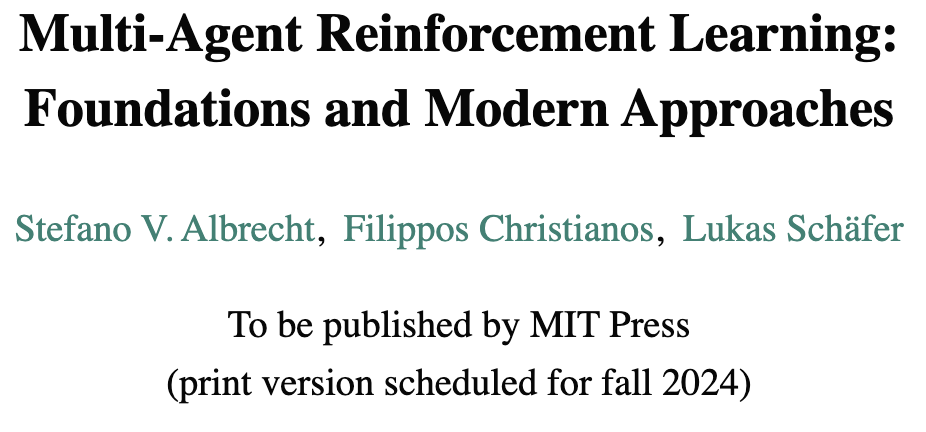
\includegraphics[width=\textwidth,height=.8\textheight,keepaspectratio]{images/1_MARL_book.png}
            
              \label{fig:enter-label}
            \end{figure}
          \end{column}
        
        \hspace{20pt}
            
          % Column for the text
            \begin{column}{0.45\textwidth}
	        \small

                This lecture is based on \textit{Multi-Agent Reinforcement Learning: Foundations and Modern Approaches} by Stefano V. Albrecht, Filippos Christianos and Lukas Sch\"afer
                
                \vspace{20pt}
                
                The book can be downloaded for free at \textcolor{blue}{\href{https://www.marl-book.com/}{www.marl-book.com}}.
            \end{column}
        
        \end{columns}
    \end{frame}
}

\newcommand{\leoslide}{
  \author{Stefano V. Albrecht, Filippos Christianos, Lukas Sch\"afer \\ Slides by: Leonard Hinckeldey}
}

\newcommand{\otherslide}{
  \author{Stefano V. Albrecht, Filippos Christianos, Lukas Sch\"afer}
}
	
\title{Multi-Agent Reinforcement Learning}
\date{}

\hypersetup{
  pdfsubject = {Multi-Agent Reinforcement Learning},
}

\otherslide

\subtitle{Multi-Agent Reinforcement Learning: Foundational Algorithms}

\begin{document}

\maketitle

\introslide

\begin{frame}{\outline}
    \blist
        \item Dynamic Programming for Games: Value Iteration
        \item Temporal-Difference Learning for Games: Joint-Action Learning
        \item Agent Modeling
        \item Policy-Based Learning
        \item No-Regret Learning
    \elist
\end{frame}

\begin{frame}{Dynamic Programming for Games: Value Iteration}
    Shapley (1953) proposed \e{value iteration} to compute \e{minimax} joint policy in zero-sum stochastic games with two agents
    \blist
        \itemsep=15pt
        \item Algorithm makes two sweeps over states $\st \in \St$ and agents $i \in \Ag$: \\[10pt]
            \begin{center}
                \imgh{images/SG-value-iter.pdf}{0.3}
            \end{center}
        \item Converges to minimax values $V_i^*(\st)$ of the stochastic game
    \elist
\end{frame}

\begin{frame}[t]{Value Iteration Pseudocode}
    \balg{Value iteration for stochastic games}{vi}
        \State Initialize: $V_i(s) = 0$ for all $\st \in \St$ and $i \in \Ag$
        \State Repeat until all $V_i$ have converged:
            \pause
        \ForAll{states $\st \in \St$, agents $i \in \Ag$, joint actions $\jac \in \Ac$}
        \bmath
            M_{\st,i}(\jac) \gets \sum_{\st' \in \St} \Stf(\st' \mid \st,\jac) \left[ \Rew_i(\st,\jac,\st') + \dsc V_i(\st') \right]
        \emath
        \EndFor
            \pause
        \ForAll{states $\st \in \St$, agents $i \in \Ag$}
        \bmath
            \hspace{10pt} V_i(\st) \gets \gval_i( M_{\st,1},...,M_{\st,n}) \hspace{10pt}\textit{// Minimax value for agent $i$}
        \emath
        \EndFor
    \ealg
\end{frame}

\begin{frame}{Obtaining Minimax Policies for the Stochastic Game}
    To obtain minimax policies $\pol_1,...,\pol_n$ for the \e{stochastic game}:
    \blist
        \item Given converged state minimax values $V_i^*$ and a state $\st$
        \item Construct the normal-form game $M^*_{s,1},...,M^*_{s,n}$
        \item Compute the minimax policies $\pol^*_1,...,\pol^*_n$ of this \e{normal-form game}
        \item Set action probabilities $\pol_i(a_i | s) \gets \pol^*_i(a_i)$ for all $\ac_i \in \Ac_i$
    \elist
\end{frame}

\begin{frame}{From Dynamic Programming to Temporal-Difference Learning}
    \begin{problembox}
        Dynamic programming requires full knowledge of game
        \blist
            \item Including reward functions $\Rew_i$ and state transition function $\Stf$
            \item May not be available!
        \elist
    \end{problembox}
    Can we \e{\it learn} equilibrium joint policy via \e{temporal-difference learning}?
\end{frame}

\begin{frame}[b]{Temporal-Difference Learning for Games: Joint-Action Learning}
    \only<1>{\imgh{images/MARL-loop-JAL-a.pdf}{0.65}}
    \only<2>{\imgh{images/MARL-loop-JAL-b.pdf}{0.82}}
    \only<3>{\imgh{images/MARL-loop-JAL-c.pdf}{0.82}}
\end{frame}

\begin{frame}{Temporal-Difference Learning for Games: Joint-Action Learning}
    \begin{problembox}
        $Q_i(s,a_1,...,a_n)$ is not enough to find optimal action for agent $i$
        \blist
            \item Cannot evaluate $\max_{a_i} Q_i(s,a_1,...,a_n)$
            \listtab Optimal action depends on actions of other agents!
        \elist
        \pause
        We have to define:
        \begin{enumerate}
            \item How to select action from $Q_i$?
            \item How to update $Q_i$?
        \end{enumerate}
    \end{problembox}
\end{frame}

\begin{frame}[t]{Joint-Action Learning with Game Theory}
    \fat{Idea:} joint-action value functions define a \e{normal-form game}: \\[5pt]
    \blist
        \itemsep=10pt
        \item<1-> Each agent stores Q-function $Q_j$ for every agent $j \in \Ag$ \\
            (assumes agents can observe all agents' actions and rewards)
        \item<2-> Define reward functions for normal-form game in state $s$ as 
        \bmath
            \Rew_j(\ac_1,...,\ac_n) = Q_j(\st,\ac_1,...,\ac_n)
        \emath
        \item<3-> We can {\it solve} the normal-form game defined by
        \bmath
            \Gamma_s = \Big ( \Rew_1 = Q_1(s,\cdot), \cdots, \Rew_n = Q_n(s,\cdot) \Big )
        \emath
    \elist
\end{frame}

\begin{frame}{Joint-Action Learning with Game Theory}
    \e{\bf Solution} of $\Gamma_s$ is a joint policy $\pol_s^* = (\pol_{s,1}^*,...,\pol_{s,n}^*)$ with certain properties
    \blist
        \item e.g. compute minimax solution or Nash equilibrium of $\Gamma_s$
        \listtab Use $\pol_{s,i}^*$ to select action for agent $i$
    \elist
    
    \vspace{1.5em}
    \pause
    
    \e{\bf Value} of $\Gamma_s$ for agent $j$ is its expected reward under joint policy $\pol_s^*$
    \bmath
        \gval_j(\Gamma_{\st}) = \sum_{\ac \in \Ac} Q_j(\st,\ac) \, \pol^*_{\st}(\ac)
    \emath
    \listtab Update $Q_j$ towards update target: \ $\rew_j + \gamma \, \gval_j(\Gamma_{s'})$
\end{frame}

\begin{frame}[t]{JAL-GT Pseudocode}
    \balg{Joint-action learning with game theory (JAL-GT)}{jal-gt}
    \Statex {\it // Algorithm controls agent $i$}
    \State Initialize: $Q_j(\st,\ac) = 0$ for all $j \in \Ag$ and $\st \in \St, \ac \in \Ac$
    \State Repeat for every episode:
    \For{$t = 0,1,2,...$}
        \State Observe current state $\st^t$
        \State With probability $\epsilon$: choose random action $\ac_i^t$
        \State Otherwise: solve $\Gamma_{\st^t}$ to get policies $(\pol_1,...,\pol_n)$, then sample action $\ac_i^t \sim \pol_i$
        \State Observe joint action $\ac^t = (\ac^t_1,...,\ac^t_n)$, rewards $\rew^t_1,...,\rew^t_n$, next state $\st^{t+1}$
        \ForAll{$j \in \Ag$}
            \State $Q_j(\st^t,\ac^t) \gets Q_j(\st^t,\ac^t) + \alpha \left[ \rew^t_j + \dsc \gval_j(\Gamma_{\st^{t+1}}) - Q_j(\st^t,\ac^t) \right]$
        \EndFor
    \EndFor
    \ealg
\end{frame}

\begin{frame}{Minimax-Q, Nash-Q, CE-Q}
    \fat{Minimax-Q} solves $\Gamma_s$ via minimax solution (Littman, 1994)
    \blist
        \item Converges to unique minimax values in two-agent zero-sum stochastic games
        \item Minimax profile can be computed with linear programming (LP)
    \elist
    \fat{Nash-Q} solves $\Gamma_s$ via Nash equilibrium (Hu and Wellman, 2003) \\
    \fat{CE-Q} solves $\Gamma_s$ via correlated equilibrium (Greenwald and Hall, 2003)
    \blist
        \item Converges to equilibrium under highly restrictive conditions % on sequence of normal-form games
            \listtab Problem: often no unique equilibrium value in general-sum games % this makes the TD targets in fact ill-defined
        \item Compute CE with LP, compute NE with quadratic programming
    \elist
\end{frame}

\begin{frame}[t]{Example: Minimax-Q in Grid Soccer (Littman, 1994)}
    \begin{center}
        \imgw{images/minimax_soccer.pdf}{0.70}
    \end{center}
    \blist
        \item Episodes start in left state with random ball assignment
        \item Agent wins episode if it moves the ball into opponent goal
        \item Agent loses ball to opponent if it moves into opponent's location
    \elist
    Against {\it unknown} opponent, optimal policy must randomise (right state; why?) % because any deterministic choice can always be blocked
\end{frame}

\begin{frame}[t]{Example: Minimax-Q in Grid Soccer (Littman, 1994)}
    \begin{center}
        \only<1>{\imgw{images/minimax_soccer_results_a.png}{0.6}}
        \only<2>{\imgw{images/minimax_soccer_results_b.png}{0.6}}
        \only<3>{\imgw{images/minimax_soccer_results_c.png}{0.6}}
    \end{center}
    \small
    \only<1>{
    \blist
        \itemsep=0pt
        \item random: uniform-random opponent policy
        \item hand-built: manual opponent policy
        \item optimal: Q-learning opponent policy trained against final policy of minimax Q / independent Q
    \elist}
    \only<2>{
    \blist
        \item minimax Q learns ``safe'' policy that works against any opponent
        \listtab minimax policy guarantees minimum average 50\% win
        \item lower \% win against optimal because minimax Q did not fully converge during training, so could be exploited by optimal opponent
    \elist}
    \only<3>{
        \begin{problembox}
            \blist
                \item Independent Q-learning can learn strong performance
                \item {\bf But:} overfits to opponent, does not generalise well to other opponents
                    \listtab ``optimal'' opponent exploits deterministic policy learned by independent Q-learning, resulting in 0\% wins
            \elist
            \vspace{-1em}
        \end{problembox}
    }
\end{frame}

\begin{frame}{Agent Modeling \& Best Response}
    Game theory solutions are \e{normative}: they {\it prescribe} how agents {\it should} behave
    \blist
        \item e.g. minimax assumes worst-case opponent
    \elist
    \pause
    What if agents don't behave as prescribed by solution?
    \blist
        \item e.g. minimax-Q was unable to exploit hand-built opponent in soccer example
    \elist
    \pause
    Other approach: \e{\bf agent modeling with best response}
    \blist
        \item Learn models of other agents to predict their actions
        \item Compute optimal action (best response) against agent models
    \elist
\end{frame}

\begin{frame}[t]{Agent Modeling}
    \center
    \imgw{images/chapter6/agentmodel.pdf}{0.90} \\[1.5em]
    Many kinds of agent modeling: \\[0.7em]
    \bcol
        \col{0.35}
            \blist
                \itemsep=1pt
                \item Policy reconstruction
                \item Type-based reasoning
                \item Classification
                \item Plan recognition
            \elist
        \col{0.35}
            \blist
                \itemsep=1pt
                \item Recursive reasoning
                \item Graphical methods
                \item Group modeling
                \item Implicit modeling
            \elist
    \ecol
    \vspace{8pt}
    \scriptsize{S. Albrecht, P. Stone. \bf Autonomous Agents Modelling Other Agents: A Comprehensive Survey and Open Problems.} {\it Artificial Intelligence}, 2018
\end{frame}

\begin{frame}{Policy Reconstruction \& Best Response}
    \fat{Policy reconstruction:} learn model $\hat{\pi}_j \approx \pi_j$ from past observed actions \\[1em]

    In general, can train model with \e{supervised learning} on data $\{(\st^\tau,\ac_j^\tau)\}_{\tau=1}^{t-1}$
    \blist
        \item E.g. look-up table, neural network, finite state machine, ...
        \item Model should support incremental updating
    \elist

    \vspace{5pt}
    \pause
    
    Given models for other agents $\agmod_{-i} = \{ \agmod_j \}_{j \neq i}$, compute \e{best response}
    \bmath
	\pol_i \in \br_i(\agmod_{-i})
    \emath
\end{frame}

\begin{frame}{Fictitious Play}
    \e{Fictitious play} (Brown 1951) algorithm for non-repeated normal-form games

    \vspace{5pt}
    
    Each agent $i$ models other agents $j$ as stationary distribution:
    \bmath
	\agmod_j(\ac_j) =\frac{C(\ac_j)}{\sum_{\ac'_j \in \Ac_j} C(\ac'_j)}
    \emath
    $C(\ac_j)$ is number of times agent $j$ chose action $\ac_j$ in prior episodes

    \vspace{5pt}
    \pause
    
    In each episode, agents choose best-response action:
    \bmath
	\br_i(\agmod_{-i}) = \arg\max_{\ac_i \in \Ac_i} \sum_{\ac_{-i} \in \Ac_{-i}} \Rew_i( \con{\ac_i,\ac_{-i}} ) \prod_{j \,\neq\, i} \agmod_j(\ac_j)
    \emath
\end{frame}

\begin{frame}{Fictitious Play Convergence}
    \begin{graytitlebox}{Fictitious Play Convergence}
        \blist
            \itemsep=10pt
            \item<1-> If agents' actions converge, then the converged actions form a NE
            \item<2-> If in any episode the agents' actions form a NE, then they will always remain in the equilibrium
            \item<3-> If empirical distribution of agents' actions converges, then the distributions converge to a NE
            \item<4-> The empirical distributions converge in several game classes, e.g. in two-agent zero-sum finite games
        \elist
    \end{graytitlebox}
\end{frame}

\begin{frame}[t]{Fictitious Play in Rock-Paper-Scissors}
    \centering
    \imgh{images/chapter6/fp_empirical_distribution_rps.pdf}{0.9}
\end{frame}

\begin{frame}{Fictitious Play in Rock-Paper-Scissors}
    \centering
    \imgh{images/chapter6/fp_rps_table.pdf}{0.8}
\end{frame}
 
\begin{frame}[t]{Joint-Action Learning with Agent Modeling}
    Extend fictitious play approach to \e{stochastic games} by using \e{joint-action learning with agent models}

    \pause
    
    Agents models other agents $j$, this time conditioned on states $\st$:
    \bmath
	\agmod_j(\ac_j \mid \st) = \frac{C(\st,\ac_j)}{\sum_{\ac'_j \in \Ac_j} C(\st,\ac'_j)}
    \emath

    \pause

    Given models $\{ \agmod_j \}_{j \neq i}$, action values are defined as:
    \bmath
	\amval_i(\st,\ac_i) = \sum_{\ac_{-i} \in \Ac_{-i}} Q_i(\st, \con{\ac_i,\ac_{-i}}) \prod_{j \neq i} \agmod_j(\ac_j \mid \st)
    \emath
    \listtab Use $\amval_i$ to select optimal actions and as learning update targets
\end{frame}

\begin{frame}{JAL-AM Pseudocode}
    \balg{Joint-action learning with agent modeling (JAL-AM)}{jal-am}
        \State Initialize:
        \State \quad $Q_i(\st,\ac) = 0$ for all $\st \in \St, \ac \in \Ac$
        \State \quad Agent models $\agmod_j(\ac_j \mid \st) = \frac{1}{|\Ac_j|}$ for all $j \neq i, \ac_j \in \Ac_j, \st \in \St$
        \State Repeat for every episode:
        \For{$t = 0,1,2,...$}
        \State Observe current state $\st^t$
        \State With probability $\epsilon$: choose random action $\ac^t_i$
        \State Otherwise: choose best-response action $\ac^t_i \in \arg\max_{\ac_i} \amval_i(\st^t,\ac_i)$
        \State Observe joint action $\ac^t = (\ac^t_1,...,\ac^t_n)$, reward $\rew^t_i$, next state $\st^{t+1}$
        \State Update agent models $\agmod_j$ with new observations (e.g., $(\st^t,\ac^t_j)$)
        \State $Q_i(\st^t,\ac^t) \gets Q_i(\st^t,\ac^t) + \alpha \left[ \rew^t_i + \dsc \max_{\ac'_i} \amval_i(\st^{t+1},\ac'_i)  - Q_i(\st^t,\ac^t) \right]$
        \EndFor
    \ealg
\end{frame}

\begin{frame}{JAL-AM in Level-Based Foraging}
    \raisebox{2em}{\imgw{images/chapter6/tabular_marl_lbf.pdf}{0.3}}
    \hfill
    \imgw{images/chapter6/tabular_marl_lbf_returns_all.pdf}{0.6}
\end{frame}

\begin{frame}{Policy-Based Learning}
    All algorithms so far derive policies from learned \e{action-value functions}
    \blist
        \item Has important limitations, e.g. algorithms using best-response actions from values (e.g. fictitious play, JAL-AM) cannot represent probabilistic equilibria
        \item Fictitious play unable to represent uniform-random NE in Rock-Paper-Scissors
    \elist
    \pause
    \e{\bf Policy-based learning} instead uses learning data to directly optimise policies
    \blist
        \item Use {\it parameterised policies} that are differentiable
        \item Use {\it gradient-ascent techniques} to optimise parameters
        \listtab Can directly learn action probabilities in policies!
    \elist
\end{frame}

\begin{frame}{Gradient Ascent in Expected Reward}
    \fat{Gradient-ascent learning} in non-repeated \nfgs with two agents $i,j$ and two actions

    Reward matrices:
    \bmath
	\Rew_i = \bra{cc}{
		r_{1,1} & r_{1,2} \\
		r_{2,1} & r_{2,2}
	} \hspace{2em}
	\Rew_j = \bra{cc}{
		c_{1,1} & c_{1,2} \\
		c_{2,1} & c_{2,2}
	}
    \emath

    \vspace{7pt}

    Policies with parameters $\alpha,\beta \in [0,1]$:
    \bmath
	\pol_i = ( \alpha , 1-\alpha ) \hspace{2em} \pol_j = (\beta , 1-\beta)
    \emath
\end{frame}

\begin{frame}[t]{Gradient Ascent in Expected Reward}
    Update policy in direction of gradient in expected reward using step size $\step > 0$:
    \begin{align*}
    	\alpha^{k+1} & = \alpha^k + \step \der{\exret_i(\alpha^k,\beta^k)}{\alpha^k} \\
    	\beta^{k+1} & = \beta^k + \step \der{\exret_j(\alpha^k,\beta^k)}{\beta^k}
    \end{align*}
    Partial derivative of an agent's expected reward with respect to its policy:
    \begin{align*}
    	\der{\exret_i(\alpha,\beta)}{\alpha} & = \beta u + (r_{1,2} - r_{2,2}) \\
    	\der{\exret_j(\alpha,\beta)}{\beta} & = \alpha u' + (c_{2,1} - c_{2,2}).
    \end{align*}
    where $u = r_{1,1} - r_{1,2} - r_{2,1} + r_{2,2}$ and $u' = c_{1,1} - c_{1,2} - c_{2,1} + c_{2,2}$
\end{frame}

\begin{frame}{Learning Dynamics of Infinitesimal Gradient Ascent}
    What joint policy will agents converge to?
    \listtab Can analyse learning dynamics via dynamical systems theory!

    \vspace{10pt}
    
    \e{Infinitesimal Gradient ascent (IGA)}: use infinitesimal step size $\step \to \infty$

    Joint policy given by $(\alpha(t),\beta(t))$ will follow continuous trajectory according to differential equation:
    \bmath
	\bra{c}{
		\der{\alpha}{t} \\ \der{\beta}{t}
	} = \underbrace{ \bra{cc}{
		0 & u \\ u' & 0
	}}_{F} \bra{c}{
		\alpha \\ \beta
	} + \bra{c}{
		(r_{1,2} - r_{2,2}) \\
		(c_{2,1} - c_{2,2})
	}
    \emath
\end{frame}

\begin{frame}[t]{Learning Dynamics of Infinitesimal Gradient Ascent}
    Learning dynamics of $(\alpha,\beta)$ will follow one of three types of trajectories: \\[10pt]
    \begin{figure}
    \visible<1->{
    \begin{subfigure}[t]{0.3\textwidth}
        \centering
        \imgw{images/chapter6/iga_noninvert.pdf}{1}
        \caption{$F$ not invertible}
    \end{subfigure}}
    \hfill
    \visible<2->{
    \begin{subfigure}[t]{0.3\textwidth}
        \centering
        \imgw{images/chapter6/iga_real.pdf}{1}
        \caption{$F$ has purely real eigenvalues}
    \end{subfigure}}
    \hfill
    \visible<3->{
    \begin{subfigure}[t]{0.3\textwidth}
        \centering
        \imgw{images/chapter6/iga_imaginary.pdf}{1}
        \caption{$F$ has purely imaginary eigenvalues}
    \end{subfigure}}
    \end{figure}
\end{frame}

\begin{frame}{IGA Convergence}
    \begin{graytitlebox}{IGA Convergence (Singh, Kearns, Mansour 2000)}
        % \bblock{IGA Convergence (Singh, Kearns, Mansour 2000)}
        \blist
            \itemsep=10pt
    	\item<1-> $(\alpha,\beta)$ does not converge in all cases
    	\item<2-> If $(\alpha,\beta)$ does not converge, then average rewards during learning converge to expected rewards of some NE
    	\item<3-> If $(\alpha,\beta)$ converges, then converged joint policy is a NE
        \elist
        % \eblock
    \end{graytitlebox}
\end{frame}

\begin{frame}{Win or Learn Fast -- Variable Learning Rate}
    By using a variable step size $\step$, we can ensure that IGA policies {\it always} converge to NE

    \vspace{5pt}

    \e{Win or Learn Fast (WoLF):} (Bowling and Veloso 2002)
    \blist
        \item learn fast (use larger $\step$) when ``losing''
        \item learn slow (use smaller $\step$) when ``winning''
    \elist
    Winning/losing depends on current expected reward compared to NE rewards
\end{frame}

\begin{frame}{Win or Learn Fast -- Variable Learning Rate}
    Modify learning rule (analogous for agent $j$):
    \bmath
	\alpha^{k+1} = \alpha^k + l_i^k \step  \der{\exret_i(\alpha^k,\beta^k)}{\alpha^k}
    \emath
    with variable step size $l_i^k \in [l_{\min},l_{\max}] > 0$
    \bmath
	l_i^k = \left\{
		\begin{array}{llr}
			l_{\min} & \text{if } \exret_i(\alpha^k,\beta^k) > \exret_i(\alpha^e,\beta^k) & \text{(winning)} \\
			l_{\max} & \text{otherwise } & \text{(losing)}
		\end{array}
		\right.
    \emath
    where $\alpha^e$ is a policy from some NE
\end{frame}

\begin{frame}{WoLF-IGA Convergence}
    \bcol
        \col{0.6}
            IGA does not converge if $F$ is invertible and has imaginary eigenvalues \\[3pt]
            \blist
                \item In WoLF-IGA, trajectories of $(\alpha,\beta)$ are piecewise elliptical, each quadrant tightens ellipse by factor $\sqrt{\frac{l_{\min}}{l_{\max}}} < 1$
                \item Using variable learning rate, WoLF-IGA converges!
            \elist
            WoLF-IGA guaranteed to learn NE in two-agent two-action \nfg
        \col{0.35}
            \imgw{images/chapter6/iga_wolf.pdf}{1}
    \ecol
\end{frame}

\begin{frame}{Win or Learn Fast with Policy Hill Climbing (WoLF-PHC)}
    \e{WoLF-PHC} algorithm (Bowling and Veloso 2002) applies WoLF principle in stochastic games:
    \blist
        \item Can learn in general-sum games with any number of agents and actions
        \item Does not require knowledge of reward functions and policies
    \elist
    To determine winning/losing, it compares average reward of current policy $\pol_i$ to ``average'' policy $\avgpol_i$ over past policies:
    \bmath
	\delta = \left\{ \begin{array}{rl}
		l_w & \text{if } \sum_{\ac_i'} \pol_i(\ac_i' \mid \st) Q(\st,\ac_i') \,>\, \sum_{\ac_i'} \avgpol_i(\ac_i' \mid \st) Q(\st,\ac_i') \\
		l_l & \text{otherwise}
	\end{array} \right.
    \emath
\end{frame}

\begin{frame}[t]{WoLF-PHC in Rock-Paper-Scissors}
    \centering
    \imgh{images/chapter6/wolfphc_rps_own.pdf}{0.9}
\end{frame}

\begin{frame}{No-Regret Learning}
    JAL-GT and JAL-AM algorithms use solution concepts and agent modeling to learn joint policies

    \vspace{5pt}
    
    \fat{Now:} \e{no-regret learning} algorithms that use regret definitions to learn policies
    \blist
        \item We consider two simple {regret matching} algorithms (Hart and Mas-Colell, 2000)
        \item In \nfgs, their empirical action distributions converge to set of (coarse) correlated equilibrium
    \elist
\end{frame}

\begin{frame}[t]{Unconditional Regret Matching}
    \e{Unconditional regret matching:} compute action probabilities proportional to (positive) average {\it unconditional} regrets of actions $\ac_i \in \Ac_i$
    \bmath
        \regret_i^z(\ac_i) = \sum_{e=1}^{z} \left[ \Rew_i( \con{ \ac_i, \jac^e_{-i}} ) - \Rew_i( \jac^e ) \right]
    \emath
    $\ac^e$ is joint action from past episodes $e = 1,...,z$.
    
    Each agent $i$ starts with a random initial policy $\pol_i^1$, then update $\pol_i^z$ to
    \bmath
	\pol_i^{z+1}(\ac_i) = \frac{ [ \avgreg_i^z(\ac_i) ]_+}{\sum_{\ac'_i \in \Ac_i} [ \avgreg_i^z(\ac'_i) ]_+} \quad\text{ with } \avgreg_i^z(\ac_i) = \frac{1}{z} \regret_i^z(\ac_i)
    \emath
    where $[x]_+ = \max[x,0]$. 
\end{frame}

\begin{frame}[t]{Conditional Regret Matching}
    \e{Conditional regret matching:} compute action probabilities proportional to (positive) average {\it conditional} regrets with respect to most recent selected action $\ac'_i$
    \bmath
	\regret_i^z(\ac'_i,\ac_i) = \sum_{e : \ac_i^e = \ac'_i} \left[ \Rew_i( \con{ \ac_i, \jac^e_{-i}} ) - \Rew_i( \jac^e ) \right]
    \emath

    Each agent $i$ starts with a random initial policy $\pol_i^1$, then update $\pol_i^z$ to
    \bmath
        \pol_i^{z+1}(\ac_i) = \left\{ \begin{array}{ll}
            \frac{1}{\eta} [\avgreg_i^z(\ac_i^z,\ac_i)]_+ & \text{if } \ac_i \neq \ac_i^z \\[5pt]
            1 - \sum_{\ac'_i \neq \ac_i^z} \pol_i^{z+1}(\ac'_i) & \text{otherwise}
        \end{array} \right. \quad\text{ with } \avgreg_i^z(\ac'_i,\ac_i) = \frac{1}{z} \regret_i^z(\ac'_i,\ac_i)
    \emath
    where $\eta > 2 \cdot \max_{\jac \in \Ac} |\Rew_i(\jac)| \cdot (|\Ac_i| - 1)$ is a parameter.
\end{frame}

\begin{frame}{Regret Matching Convergence}
    In both types of regret matching, the average regrets are bounded by $\kappa \frac{1}{\sqrt{z}}$ for some constant $\kappa > 0$
    \blist
        \item For infinite episodes $z \to \infty$, the average regrets $\avgreg_i^z$ will be at most $0$
        \listtab Thus, agents learn no-regret joint policy!
        \item Does not require any assumptions about the actions of other agents
    \elist
    Empirical action distributions converge to:
    \blist
        \item Unconditional regret matching $\rightarrow$ coarse correlated equilibrium
        \item Conditional regret matching $\rightarrow$ correlated equilibrium
    \elist
\end{frame}

\begin{frame}{Unconditional Regret Matching in \rps}
    \begin{figure}
        \begin{subfigure}[t]{0.45\textwidth}
            \imgw{images/chapter6/regmat_rps_policy2.pdf}{1}
            \caption{Policies $\pol_i^z$}
        \end{subfigure}
        \hfill
        \visible<2->{
        \begin{subfigure}[t]{0.45\textwidth}
            \imgw{images/chapter6/regmat_rps_empdist2.pdf}{1}
            \caption{Empirical distributions $\empdis_i^z$}
        \end{subfigure}}
    \end{figure}
\end{frame}

\begin{frame}{Unconditional Regret Matching in \rps}
    \begin{figure}[t]
	\begin{subfigure}[t]{0.48\textwidth}
            \imgw{images/chapter6/regmat_rps_regret1.pdf}{1}
		\caption{Agent 1}
	\end{subfigure}
	\hfill
	\begin{subfigure}[t]{0.48\textwidth}
            \imgw{images/chapter6/regmat_rps_regret2.pdf}{1}
		\caption{Agent 2}
	\end{subfigure}
    \end{figure}
\end{frame}

\begin{frame}{Summary}
    \fat{We covered:}
    \blist
        \item Value iteration for stochastic games
        \item Joint-action value learning algorithms
        \blisttab
            \item JAL-GT: temporal-difference learning with game theory solution concepts
            \item JAL-AM: temporal-difference learning with agent models and best responses
        \elisttab
        \item Learning policies by optimising policy parameters with gradient ascent
        \item Learning policies by minimising notions of regret
    \elist

    \fat{Next we'll cover:}
    \blist
        \item Deep learning
    \elist
\end{frame}

\end{document}
